\documentclass[../main.tex]{subfiles}

\begin{document}
\chapter{Drivers of Antarctic Land Ice}
\label{chap:land_ice}
In chapter \ref{chap:temp_and_ice}, we found that temperature is significant for our understanding of the trends in Antarctic \gls{sic} over the last 40 years. However we found that the relationship between temperature and land ice is not as strong. To understand this we will have to do some more calculations.

We want to consider a range of variables which could be impacting land ice in Antarctica. We will include temperature again for completeness. Wind speed is linked to atmospheric circulations which move clouds and thermal energy around the continent. Cloud cover has also been linked to behaviours in the land ice. \textcolor{red}{add appropriate citations here}. 

Let's start by looking at the behaviour of land ice.

\section{Land ice trends and variability}
 \begin{figure}[H]
     \centering
     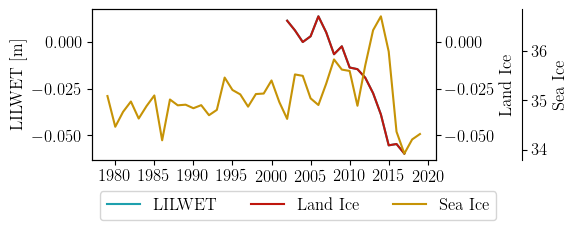
\includegraphics{images/2021w4/trends/lres/LIC.png}
     \caption{Mean value of \gls{lilwet} from 2002 to 2019.}
     \label{fig:lilwet_mean}
 \end{figure}

The simplest thing we can do at this point is to compare the mean time series of this with different variables.

\section{Comparing land ice with different variables}
For the first step in analysis here we plotted the mean values for both land ice and other environmental variables, considering only the grid points where we have data for land ice.

% \begin{figure}
%      \centering
%      \begin{subfigure}[b]{\textwidth}
%          \centering
%          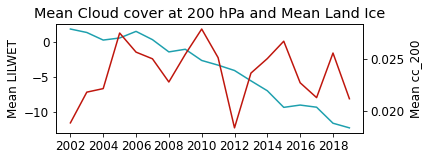
\includegraphics[width=\textwidth]{images/2021w2/lres/timeseries_cc_200_lic}
%          \caption{Mean cloud cover at 200 hPa}
%      \end{subfigure}
%      \hfill
%      \begin{subfigure}[b]{\textwidth}
%          \centering
%          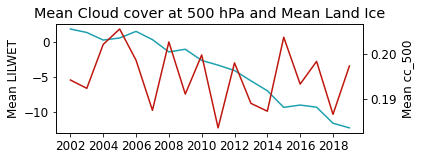
\includegraphics[width=\textwidth]{images/2021w2/lres/timeseries_cc_500_lic}
%          \caption{Mean cloud cover at 500 hPa}
%      \end{subfigure}
%      \hfill
%      \begin{subfigure}[b]{\textwidth}
%          \centering
%          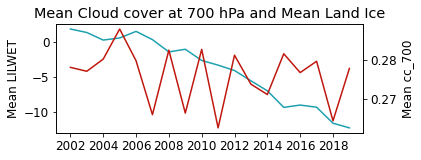
\includegraphics[width=\textwidth]{images/2021w2/lres/timeseries_cc_700_lic}
%          \caption{Mean cloud cover at 700 hPa}
%      \end{subfigure}
%         \caption{Three simple graphs}
%         \label{fig:three graphs}
% \end{figure}
\section{}


\end{document}